\section{\emph{Efficient Unidirectional Proxy Re-Encryptation}}
\label{recifragem:EU-PRE}
O \emph{Efficient Unidirectional Proxy Re-Encryptation}, o qual a partir daqui o iremos referenciá-lo com EU-PRE, possui seis algoritmos principais: \emph{configuração},\emph{geração de chaves}, \emph{cifragem},\emph{geração de chave de recifragem}, \emph{recifragem} e \emph{decifragem}. Que são detalhados, segundo \cite{mannes2016controle}, como os seguintes:

\paragraph{Configuração:} escolher dois números primos \emph{p} e \emph{q} tal que \emph{q} | \emph{p} - 1 (\emph{q} deve ser divisor de (p-1)), o parâmetro $\ell_0$ para o tamanho da mensagem, o parâmetro de segurança $\ell_1$ e um gerador \emph{g} do grupo $\mathbb{G}$ (um subgrupo de $\mathbb{Z^*_q}$ de ordem $q$). Além desses parâmetros, o sistema utiliza quatro funções de $hash$:$H_1 : {\left\{0,1\right\}}^{\ell_0} \times {\left\{0,1\right\}}^{\ell_1} \rightarrow \mathbb{Z^*_q}$, $H_2: \mathbb{G} \rightarrow {\left\{0,1\right\}}^{\ell_0 + \ell_1}$, $H_3 : {\left\{0,1\right\}}^{*} \rightarrow \mathbb{Z^*_q}$, $H_4 :  \mathbb{G} \rightarrow \mathbb{Z^*_q}$ . Os parâmetros públicos do sistema são: $\left(\emph{q},\mathbb{G},\emph{g},H_1,H_2,H_3,H_4,\ell_0,\ell_1\right)$.

\paragraph{Geração de chaves:} O conjunto de chaves do EU-PRE é composto por dois pares de chaves públicas-privadas para cada usuário do sistema. Essa caracaterística é introduzida por \cite{chow2010efficient} para garantir que a chave privada de um usuário \emph{u}1 não seja divulgada caso o \emph{proxy} e o usuário troquem informações. Considerando um usuário \emph{u}1, as chaves privadas $\emph{sk}1_{(\emph{u}1)}$ e $\emph{sk}2_{(\emph{u}1)}$ são escolhidas aleatoriamente em $\mathbb{Z}^*_q$ e as chaves públicas são calculadas por $\emph{g}^{sk}$, assim $sk1_{\emph({u}1)}$ = $\emph{g}^{sk_{(\emph{u}1)}}\mod{p}$ e $pk2_{(u1)} = \emph{g}^{(sk1)}\mod{p}$.   

\paragraph{Cifragem:} uma mensagem $m$ é cifrada pelo usuário $u1$
com suas chaves públicas $pk1_{(u1)}$ e $pk2_{(u1)}$. Escolher $t$ a partir de $\mathbb{Z}^*_q$ e $\omega$ de tamanho $\ell_1$ e calcular $r = H_1(m,\omega)$ e $D,E$ e $F$ como segue:
\begin{equation}
    D = ({{pk1^{H_{4(pk2_{u1})}}_{(u1)}} \times pk2_{(u1)})}^t \mod{p} )
\end{equation}
\begin{equation}
    E = ({pk1^{H_{4(pk2_{(u1)})}} \times pk2_{u1} })^r\mod{p})
\end{equation}
\begin{equation}
    F = H_2(g^r\mod{p})\oplus(m\parallel \omega) 
\end{equation}

Calcular também $ r = t+r\bullet H_3(D,E,F)\mod{p}$. A saída é $(D,F,E,s)$
\paragraph{Geração de chaves de recifragem:} Para geração de chave de recifragem de $u1$ para $u2$, são necessárias as chaves privadas de $u1$ e uma das chaves públicas de $u2$,$pk2_{(u2)}$. Deve-se escolher aleatoriamente $h$ de tamanho $\ell_0$ e $\pi$ de tamanho $\ell_1$ e calcular $v = H_1(h \times \pi)$. Calcular também $V = pk2^v_{(u2)} \mod{p}$ e $W = H_2(g^v\mod{p})\oplus(h \parallel \pi)$.
A chave de recifragem é:
\begin{equation}
    rk_{u1\rightarrow u2} = \big( {(sk1_{(u1)}) \bullet H_4(pk2_{(u2)} + sk2_{(u2)})}^{-1} \mod{p-1}  \big)
\end{equation}
A saída é $(rk_{u1\rightarrow u2},V,W)$.

\paragraph{Recifragem:}
Primeiramente o \emph{proxy} deve verificar :
\begin{equation}
\label{equation:rk}
    {(pk1^{H4(pk2_{(u1)})}_{(u1)} \bullet {pk2_{(u1)}\mod{p}})}^s \mod{p} = D \bullet (E^{H_3(D,E,F)} \mod{p} )\mod{p}
\end{equation}
E caso a equação \ref{equation:rk} seja verdadeira:
\begin{equation}
\label{equation:eu-pre:recifragem}
    E' = E^{rk_{u1\rightarrow u2}} \mod{p}
\end{equation}
A saída será $(E',F,V,W)$.
\paragraph{Decifragem:} A mensagem $m$ é decifrada por $u2$ mediante sua chave privada $sk2_{(u2)}$.
Primeiramente o usuário $u2$ recupera $(h\parallel\pi)$ e $(m\parallel\omega)$ ao calcular:
\begin{equation}
    (h\parallel\pi) = W \oplus H_2(V^{sk^{-1}_{(u2)}\mod{p-1}} \mod{p})
\end{equation}
\begin{equation}
\label{equation:eu-pre:decifragem}
    (m\parallel\omega) = F \oplus H_2(E'^{h^{-1}\mod{p-1}} \mod{p})
\end{equation}
A saída é a mensagem $m$ se $V = {pk2^{H_1(h,\pi)}_{(u2)}} \mod{p}$ e $E' = g^{H_1(m,\omega)\bullet h} \mod{p}$.
Na figura \ref{figura:fluxo_eu-pre} podemos visualizar todo o processo de recifragem do EU-PRE e o fluxo sequencial de cada etapa.
\begin{figure}[H]
\caption{Fluxo de processos do EU-PRE (\cite{mannes2016controle})
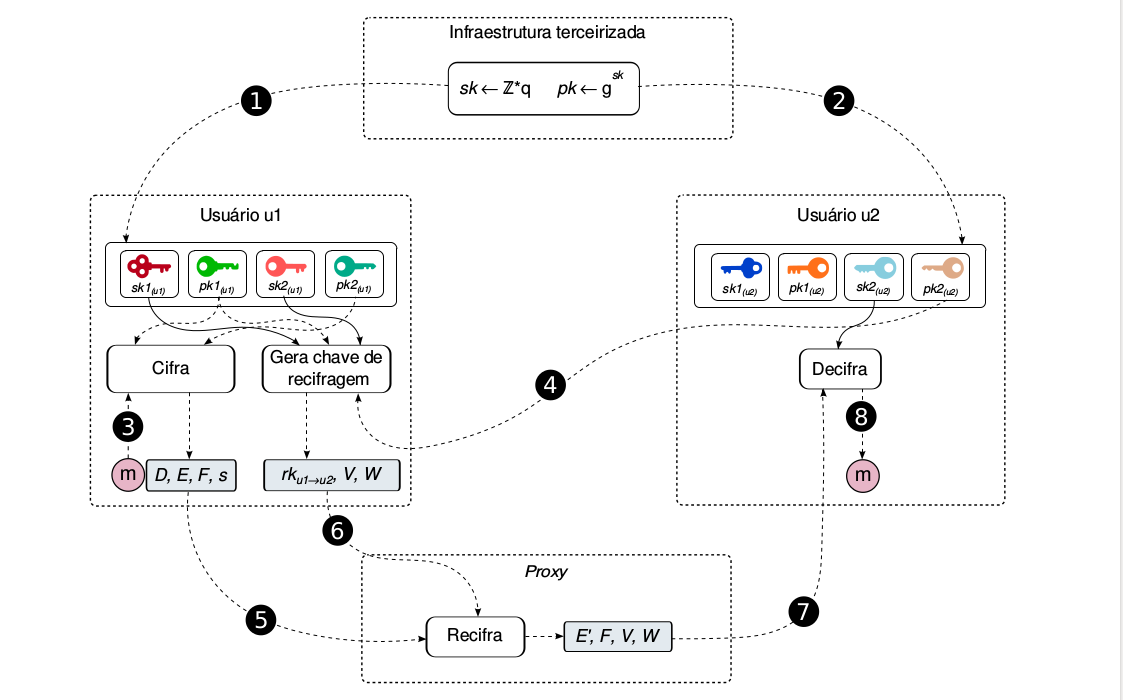
\includegraphics[height=11cm]{Figuras/fluxo_EU-PRE.png} 
\label{figura:fluxo_eu-pre}
\end{figure}

É importante salientar que no esquema de recifragrem por \emph{proxy} tradicionalmente é composto por quatro entidades: uma infraestrutura terceirizada responsável por delegar as chaves que serão utilizadas, o usuário que as delega, o \emph{proxy} e o usuário que recebe e delegação. 
Dentro desse ecosistema a divisão: Os algoritmos de configuração e geração de chaves dos usuários são executados na infraestrutura terceirizada. A cifragem e a geração de chaves de cifragem são realizadas no usuário que delega os direitos de recifragem. A recifragem é responsabilidade do \emph{proxy} e a decifragem é executada no usuário (dispositivo) que irá consumir as informações.